\section{The $\DTCWT$ Gain Layer}\label{sec:ch6:gainlayer}
To do the mixing across the $C_l$ channels at each subband, giving $C_{l+1}$
output channels, we introduce the learnable filters $g_{lp},\ g_{j,k}$:
%
\begin{align}
  g_{lp} &\in \reals[C_{l+1}\x C_l\x k_{lp}\x k_{lp}] \label{eq:ch6:glp} \\
  g_{1,1} &\in \complexes[C_{l+1}\x C_l\x k_1\x k_1] \\
  g_{1,2} &\in \complexes[C_{l+1}\x C_l\x k_1\x k_1] \\
      & \vdots \nonumber \\
  g_{J,6} &\in \complexes[C_{l+1}\x C_l\x k_J\x k_J]  \label{eq:ch6:gj6}
\end{align}
%
where the $k_j$ are the sizes of the mixing kernels. These could be $1\x 1$ for
simple gain control, or could be larger, say $3\x 3$, to do more complex
filtering on the subbands. Importantly, we can select the support size
differently for each subband.

With these gains we define the action of the gain layer $v = Gu$ to be:
\begin{align} 
  v_{lp}[f, \nn] &=  \sum_{c=0}^{C_l-1} u_{lp}[c, \nn] \conv g_{lp}[f, c, \nn] \label{eq:ch6:gain1} \\
  v_{1,1}[f, \nn] &=  \sum_{c=0}^{C_l-1} u_{1,1}[c, \nn] \conv g_{1,1}[f, c, \nn] \\
  v_{1,2}[f, \nn] &=  \sum_{c=0}^{C_l-1} u_{1,2}[c, \nn] \conv g_{1,2}[f, c, \nn] \\
                  & \vdots \nonumber \\
  v_{J,6}[f, \nn] &=  \sum_{c=0}^{C_l-1} u_{J,6}[c, \nn] \conv g_{J,6}[f, c, \nn] \label{eq:ch6:gain2}
\end{align}

To avoid ambiguity with complex conjugates we remind ourselves that for complex
signals $a, b$ the convolution $a \conv b$ is defined as $(a_r \conv b_r - a_i
\conv b_i) + j(a_r \conv b_i + a_i \conv b_r)$ (see
\autoref{sec:appE:complex_conv}).

The action of the gain layer with only a single-scale wavelet transform, $J=1$, is is shown in
\autoref{fig:ch6:block_diagrams}.

\begin{figure}[t!]
  \centering
  % \resizebox{\textwidth}{!}{\begin{tikzpicture}[%
  path image/.style={%
    path picture={%
      \node at (path picture bounding box.center) {%
        \includegraphics[height=2.0cm]{#1}
      };
    }
  }, 
  path pic/.style={%
    path picture={%
      \node at (path picture bounding box.center) {%
        \includegraphics[height=0.8cm]{#1}
      };
    }
  }, 
  scale=0.6]
  \draw (-1, 0.8, 3.5) node {\Large{$x^{(l)}$}};
  \draw (8.5, 2.5, 0) node {\Large{$u^{(l)}$}};
  \draw (9.7, 2.3, 0) node {\Large{$\conv$}};
  \draw (11, 2.5, 0) node {\Large{$g^{(l)}$}};
  \draw (15, 2.5, 0) node {\Large{$v^{(l+1)}$}};
  \draw (18.5, 2.5, 0) node {\Large{$u^{(l+1)}$}};
  \draw (25, 0.8, 3.5) node {\Large{$x^{(l+1)}$}};
  \draw[<->] (10, -1, -2) -- (10, 0.9, -2) node[near end, right] {$C_{l+1}$};

  \draw (1.0, -2.5, -3) node {bandpass};
  \draw (2.0, -2.5, 14) node {lowpass};
  \draw [decorate,decoration={brace,mirror,amplitude=10pt,raise=4pt},yshift=0pt]
    (3.8,-2.5,-8) -- (4.8,-2.5,18) node [black,midway,xshift=0.8cm];
  \draw [->, fill=gray!30,ultra thick] (0.5, -2.5, 4) -- (2.5, -2.5, 4)
    node[midway, above] {$\DTCWT$};
  \tikzcuboid{
  shiftx=-2.5cm,
  shifty=-2.5cm,
  shiftz=7,
  scale=0.5,
  anglex=0, 
  angley=90, 
  anglez=230,
  dimx=3, 
  dimy=3, 
  dimz=6,
  densityx=1, 
  densityy=1, 
  densityz=1,
  shade=false,
  emphedge=true,
  shadeopacity=0,
  emphstyle/.style={rounded corners=0.2pt,line width=0.3mm},
  front/.style={draw=blue!50!white,fill=blue!50!white},%
  right/.style={draw=blue!50!white,fill=blue!50!white},%
  top/.style={draw=blue!50!white,fill=blue!50!white},%
  drawxdims=true,
  dimxval=W,
  drawydims=true,
  dimyval=H,
  drawzdims=true,
  dimzval=C_l,
  }

  % Draw the 6 subband activations and their filters
  \foreach \i in {1,...,5} {
    \tikzcuboid{
    shiftx=6cm,
    shifty=-2.0cm,
    shiftz=-15+5*\i,
    scale=0.5,
    dimx=2, dimy=2, dimz=3,
    densityx=4, densityy=4, densityz=2,
    drawxdims=false,
    drawydims=false,
    dimzval=C_l,
    drawzdims=false,
    front/.style={draw=blue!90!white,fill=blue!90!white},%
    right/.style={draw=blue!90!white,fill=blue!90!white},%
    top/.style={draw=blue!90!white,fill=blue!90!white},%
    }
    \tikzcuboid{
    dimz=2,
    shiftx=12.0cm,
    }
    \tikzcuboid{
    shiftx=16.0cm,
    }
    \draw [->, fill=gray!30,ultra thick] (9.8+0.08*\i, -1.5, -7+2.5*\i) -- (10.8+0.08*\i, -1.5, -7+2.5*\i);
      % node[midway, above] {$\sigma_w$};
    \draw [->, fill=gray!30,ultra thick] (13.8+0.08*\i, -1.5, -7+2.5*\i) -- (14.8+0.08*\i, -1.5, -7+2.5*\i)
      node[midway, above] {$\sigma_w$};

    \tikzcuboid{
    shiftx=8.5cm,
    shifty=-1.0cm,
    shiftz=-15+5*\i,
    dimx=0.4, dimy=0.4, dimz=3,
    densityx=5, densityy=5, densityz=2,
    front/.style={draw=red!90!white,fill=red!90!white},%
    right/.style={draw=red!90!white,fill=red!90!white},%
    top/.style={draw=red!90!white,fill=red!90!white},%
    }
    \tikzcuboid{
    shifty=-1.5cm,
    }
    \tikzcuboid{
    shifty=-2.0cm,
    }
    \tikzcuboid{
    shifty=-2.5cm,
    }
    % \draw (8cm, -1.8cm, -15+5*\i) node {$\vdots$};
  }
  \tikzcuboid{
  shiftx=6cm,
  shifty=-2.0cm,
  shiftz=15,
  scale=0.5,
  dimx=2, dimy=2, dimz=3,
  densityx=4, densityy=4, densityz=2,
  dimxval=\frac{W}{2},
  drawxdims=true,
  dimyval=\frac{H}{2},
  drawydims=true,
  dimzval=C_l,
  drawzdims=true,
  front/.style={draw=blue!90!white,fill=blue!90!white},%
  right/.style={draw=blue!90!white,fill=blue!90!white},%
  top/.style={draw=blue!90!white,fill=blue!90!white},%
  }
  \tikzcuboid{
  shiftx=12.0cm,
  dimz=2,
  dimzval=C_{l+1},
  }
  \tikzcuboid{
  shiftx=16.0cm,
  drawxdims=false,
  drawydims=false,
  drawzdims=false
  }
  \draw [->, fill=gray!30,ultra thick] (9.8+6*0.08, -1.5, 8) -- (10.8+6*0.08, -1.5, 8);
    % node[midway, above] {$\sigma_w$};
  \draw [->, fill=gray!30,ultra thick] (13.8+6*0.08, -1.5, 8) -- (14.8+6*0.08, -1.5, 8)
      node[midway, above] {$\sigma_w$};
  \tikzcuboid{
  shiftx=8.5cm,
  shifty=-1.0cm,
  shiftz=15,
  dimx=0.4, dimy=0.4, dimz=3,
  drawxdims=false,
  drawydims=false,
  drawzdims=false,
  densityx=5, densityy=5, densityz=2,
  front/.style={draw=red!90!white,fill=red!90!white},%
  right/.style={draw=red!90!white,fill=red!90!white},%
  top/.style={draw=red!90!white,fill=red!90!white},%
  }
  \tikzcuboid{
  shifty=-1.5cm,
  }
  \tikzcuboid{
  shifty=-2.0cm,
  }
  \tikzcuboid{
  shifty=-2.5cm,
  }

  % Draw the lowpass activation and its set of filters
  \tikzcuboid{
  shiftx=6cm,
  shifty=-2.0cm,
  shiftz=35,
  scale=0.5,
  dimx=3, dimy=3, dimz=4,
  densityx=4, densityy=4, densityz=2,
  dimxval=W,
  drawxdims=true,
  dimyval=H,
  drawydims=true,
  dimzval=C_l,
  drawzdims=true,
  front/.style={draw=blue!50!white,fill=blue!50!white},%
  right/.style={draw=blue!50!white,fill=blue!50!white},%
  top/.style={draw=blue!50!white,fill=blue!50!white},%
  }
  \tikzcuboid{
  shiftx=12.0cm,
  dimz=2,
  drawxdims=true,
  drawydims=true,
  dimzval=C_{l+1},
  drawzdims=true
  }
  \tikzcuboid{
  shiftx=16.0cm,
  drawxdims=false,
  drawydims=false,
  drawzdims=false,
  }
  \draw [->, fill=gray!30,ultra thick] (11.2, -1.5, 17.5) -- (12.0, -1.5, 17.5);
    % node[midway, above] {$\sigma_w$};
  \draw [->, fill=gray!30,ultra thick] (15.5, -1.5, 17.5) -- (16.5, -1.5, 17.5)
    node[midway, above] {$\sigma_w$};

  \tikzcuboid{
  shiftx=9cm,
  shifty=-2.75cm,
  dimx=0.8, dimy=0.8, dimz=3,
  drawxdims=false,
  drawydims=false,
  drawzdims=false,
  densityx=5, densityy=5, densityz=2,
  front/.style={draw=red!50!white,fill=red!50!white},%
  right/.style={draw=red!50!white,fill=red!50!white},%
  top/.style={draw=red!50!white,fill=red!50!white},%
  }
  \tikzcuboid{
  shifty=-2.00cm,
  }
  \tikzcuboid{
  shifty=-1.25cm,
  }
  \tikzcuboid{
  shifty=-0.5cm,
  }
  \tikzcuboid{
  shiftx=23cm,
  shifty=-2.5cm,
  shiftz=7,
  scale=0.5,
  anglex=0, 
  angley=90, 
  anglez=230,
  dimx=3, 
  dimy=3, 
  dimz=6,
  densityx=1, 
  densityy=1, 
  densityz=1,
  shade=false,
  emphedge=true,
  shadeopacity=0,
  emphstyle/.style={rounded corners=0.2pt,line width=0.3mm},
  front/.style={draw=blue!50!white,fill=blue!50!white},%
  right/.style={draw=blue!50!white,fill=blue!50!white},%
  top/.style={draw=blue!50!white,fill=blue!50!white},%
  drawxdims=true,
  dimxval=W,
  drawydims=true,
  dimyval=H,
  drawzdims=true,
  dimzval=C_{l+1},
  }
  % \draw (0, .3, 0) node {\large{$x^{(l)}$}};
  \draw [decorate,decoration={brace,amplitude=10pt,raise=4pt},yshift=0pt]
    (16.5,-2.5,-8) -- (18,-2.5,18) node [black,midway,xshift=0.8cm];
  \draw [->, fill=gray!30,ultra thick] (19, -2.5, 4) -- (21.5, -2.5, 4)
    node[midway, above] {$\DTCWT^{-1}$};

\end{tikzpicture}
}
  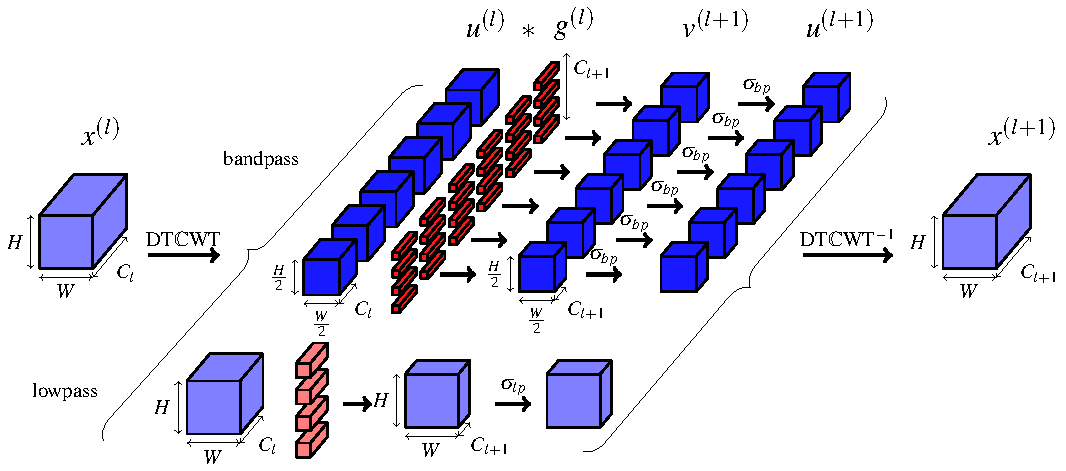
\includegraphics[width=\textwidth]{\imgpath/block_diagram_dtcwt}
  \label{fig:ch6:dtcwt_blk_diagram}
  \mycaption{Diagram of proposed method to learn in the wavelet domain}{
  Activations are shaded blue and learned parameters red. Deeper shades of blue
  and red indicate complex valued activations/weights, and lighter values
  indicate real valued activations/weights. The input $x^{(l)}\in
  \mathbb{R}^{C_l\x H\x W}$ is taken into the wavelet domain (here $J=1$) and each 
  subband is mixed independently with $C_{l+1}$ sets of convolutional filters.
  After mixing, a possible wavelet nonlinearity $\sigma_w$ is applied to the
  subbands, before returning to the pixel domain with an inverse wavelet
  transform. Note the similarity to the regular convolutional layer in
  \autoref{fig:ch2:conv_layer}.}
  \label{fig:ch6:block_diagrams}
\end{figure}

\subsection{The Output}
% \begin{figure}[t]
  % \centering
  % \begin{tikzpicture}
    \matrix (m1) [row sep=5mm, column sep=6mm,align=center,anchor=center]
	{
	%--------------------------------------------------------------------
		\node[coordinate]                  (m00) {};    &
		\node[coordinate]                  (m01) {};          &
		\node[dspsquare]                   (m02) {$A_r(z)$};          &
		\node[circle,draw,inner sep=1pt]   (m03) {\downsamplertext{M}}; &
		\node[dspnodeopen,dsp/label=above] (m04) {$U_r(z)$};          &
    \node[rectangle,draw,inner sep=2pt](m05) {$G_{r}(z)$}; &
		\node[dspnodeopen,dsp/label=above] (m06) {$V_r(z)$};          &
		\node[circle,draw,inner sep=1pt]   (m07) {\upsamplertext{M}}; &
		\node[dspsquare]                   (m08) {$S_r(z)$};          &
		\node[coordinate]                  (m09) {};          &
		\node[coordinate]                  (m0X) {};          \\
		%--------------------------------------------------------------------
		\node[]                            (m10) {$X(z)$};          &
		\node[coordinate]                  (m11) {};          &
		\node[coordinate]                  (m12) {};    &
		\node[coordinate]                  (m13) {};          &
		\node[coordinate]                  (m14) {};    &
		\node[coordinate]                  (m15) {};          &
		\node[coordinate]                  (m16) {};    &
		\node[coordinate]                  (m17) {};          &
		\node[coordinate]                  (m18) {};    &
		\node[dspadder]                    (m19) {};          &
    \node[]                            (m1X) {$Y(z)$};          \\
		%--------------------------------------------------------------------
		\node[coordinate]                  (m20) {};    &
		\node[coordinate]                  (m21) {};          &
		\node[dspsquare]                   (m22) {$A_i(z)$};          &
		\node[circle,draw,inner sep=1pt]   (m23) {\downsamplertext{M}}; &
		\node[dspnodeopen,dsp/label=below] (m24) {$U_i(z)$};          &
      \node[rectangle,draw,inner sep=2pt](m25) {$G_{r}(z)$}; &
		\node[dspnodeopen,dsp/label=below] (m26) {$V_i(z)$};          &
		\node[circle,draw,inner sep=1pt]   (m27) {\upsamplertext{M}}; &
		\node[dspsquare]                   (m28) {$S_i(z)$};          &
		\node[coordinate]                  (m29) {};          &
		\node[coordinate]                  (m2X) {};          \\
		%--------------------------------------------------------------------
  };
	\draw[dspline] (m10) -- (m11);
	\draw[dspline] (m11) -- (m01);
	\draw[dspline] (m11) -- (m21);
	\foreach \i in {0,2} {
    	\draw[dspconn] (m\i1) -- (m\i2);
    	\draw[dspconn] (m\i2) -- (m\i3);
    	\draw[dspline] (m\i3) -- (m\i4);
    	\draw[dspconn] (m\i4) -- (m\i5);
    	\draw[dspline] (m\i5) -- (m\i6);
    	\draw[dspconn] (m\i6) -- (m\i7);
    	\draw[dspconn] (m\i7) -- (m\i8);
    	\draw[dspline] (m\i8) -- (m\i9);
	}
	%\draw[dspflow] (m04) --  (m06);
	%\draw[dspflow] (m24) -- (m26);
  \draw[dspconn] (m24) -- node[draw,pos=0.7,inner sep=2pt,fill=white] {$-G_{i}(z)$} (m06);
  \draw[dspconn] (m04) -- node[draw,pos=0.7,inner sep=2pt,fill=white] {$G_{i}(z)$} (m26);
  \draw[dspconn] (m09) -- (m19);
  \draw[dspconn] (m29) -- (m19);
	\draw[dspconn] (m19) -- (m1X);
	
\end{tikzpicture}


  % \mycaption{Block Diagram of a single channel 1-D $\DTCWT$ Gain Layer}{Here we show the real and
  % imaginary trees for a single subband. Note that while it may look similar to 
  % a DWT block diagram, this diagram represents the two trees for one subband rather
  % than a single tree with a pair of subbands. The gain layer does a complex
  % multiply, using both the real and imaginary parts of the decomposed signal.
  % This preserves the shift invariance of the $\DTCWT$ for the reconstructed
  % signal $Y$.
  % }
  % \label{fig:ch6:dtcwt_gain}
% \end{figure}
\begin{figure}[t]
  \centering
  \makebox[\linewidth][c]{
  \subfloat[]{%
    % \includegraphics[width=\textwidth]{\imgpath/dtcwt_gain}
    \begin{tikzpicture}
    \matrix (m1) [row sep=5mm, column sep=6mm,align=center,anchor=center]
	{
	%--------------------------------------------------------------------
		\node[coordinate]                  (m00) {};    &
		\node[coordinate]                  (m01) {};          &
		\node[dspsquare]                   (m02) {$A_r(z)$};          &
		\node[circle,draw,inner sep=1pt]   (m03) {\downsamplertext{M}}; &
		\node[dspnodeopen,dsp/label=above] (m04) {$U_r(z)$};          &
    \node[rectangle,draw,inner sep=2pt](m05) {$G_{r}(z)$}; &
		\node[dspnodeopen,dsp/label=above] (m06) {$V_r(z)$};          &
		\node[circle,draw,inner sep=1pt]   (m07) {\upsamplertext{M}}; &
		\node[dspsquare]                   (m08) {$S_r(z)$};          &
		\node[coordinate]                  (m09) {};          &
		\node[coordinate]                  (m0X) {};          \\
		%--------------------------------------------------------------------
		\node[]                            (m10) {$X(z)$};          &
		\node[coordinate]                  (m11) {};          &
		\node[coordinate]                  (m12) {};    &
		\node[coordinate]                  (m13) {};          &
		\node[coordinate]                  (m14) {};    &
		\node[coordinate]                  (m15) {};          &
		\node[coordinate]                  (m16) {};    &
		\node[coordinate]                  (m17) {};          &
		\node[coordinate]                  (m18) {};    &
		\node[dspadder]                    (m19) {};          &
    \node[]                            (m1X) {$Y(z)$};          \\
		%--------------------------------------------------------------------
		\node[coordinate]                  (m20) {};    &
		\node[coordinate]                  (m21) {};          &
		\node[dspsquare]                   (m22) {$A_i(z)$};          &
		\node[circle,draw,inner sep=1pt]   (m23) {\downsamplertext{M}}; &
		\node[dspnodeopen,dsp/label=below] (m24) {$U_i(z)$};          &
      \node[rectangle,draw,inner sep=2pt](m25) {$G_{r}(z)$}; &
		\node[dspnodeopen,dsp/label=below] (m26) {$V_i(z)$};          &
		\node[circle,draw,inner sep=1pt]   (m27) {\upsamplertext{M}}; &
		\node[dspsquare]                   (m28) {$S_i(z)$};          &
		\node[coordinate]                  (m29) {};          &
		\node[coordinate]                  (m2X) {};          \\
		%--------------------------------------------------------------------
  };
	\draw[dspline] (m10) -- (m11);
	\draw[dspline] (m11) -- (m01);
	\draw[dspline] (m11) -- (m21);
	\foreach \i in {0,2} {
    	\draw[dspconn] (m\i1) -- (m\i2);
    	\draw[dspconn] (m\i2) -- (m\i3);
    	\draw[dspline] (m\i3) -- (m\i4);
    	\draw[dspconn] (m\i4) -- (m\i5);
    	\draw[dspline] (m\i5) -- (m\i6);
    	\draw[dspconn] (m\i6) -- (m\i7);
    	\draw[dspconn] (m\i7) -- (m\i8);
    	\draw[dspline] (m\i8) -- (m\i9);
	}
	%\draw[dspflow] (m04) --  (m06);
	%\draw[dspflow] (m24) -- (m26);
  \draw[dspconn] (m24) -- node[draw,pos=0.7,inner sep=2pt,fill=white] {$-G_{i}(z)$} (m06);
  \draw[dspconn] (m04) -- node[draw,pos=0.7,inner sep=2pt,fill=white] {$G_{i}(z)$} (m26);
  \draw[dspconn] (m09) -- (m19);
  \draw[dspconn] (m29) -- (m19);
	\draw[dspconn] (m19) -- (m1X);
	
\end{tikzpicture}


    \label{fig:ch6:fwd_pass}
    }}
   \newline
  \makebox[\linewidth][c]{
  \subfloat[]{%
    \begin{tikzpicture}
    \matrix (m1) [row sep=5mm, column sep=6mm,align=center,anchor=center]
	{
	% %--------------------------------------------------------------------
		% \node[coordinate]                  (m00) {};    &
		% \node[coordinate]                  (m01) {};          &
		% \node[dspsquare]                   (m02) {$A(z)$};          &
		% \node[circle,draw,inner sep=1pt]   (m03) {\downsamplertext{M}}; &
		% \node[dspnodeopen,dsp/label=above] (m04) {$V_r(z)$};          &
		% \node[rectangle,draw,inner sep=2pt](m05) {$G_r(z)$}; &
		% \node[dspnodeopen,dsp/label=above] (m06) {$W_r(z)$};          &
		% \node[circle,draw,inner sep=1pt]   (m07) {\upsamplertext{M}}; &
		% \node[dspsquare]                   (m08) {$C(z)$};          &
		% \node[coordinate]                  (m09) {};          &
		% \node[coordinate]                  (m0X) {};          \\
		% %--------------------------------------------------------------------
		% \node[]                            (m10) {$X(z)$};          &
		% \node[coordinate]                  (m11) {};          &
		% \node[coordinate]                  (m12) {};    &
		% \node[coordinate]                  (m13) {};          &
		% \node[coordinate]                  (m14) {};    &
		% \node[coordinate]                  (m15) {};          &
		% \node[coordinate]                  (m16) {};    &
		% \node[coordinate]                  (m17) {};          &
		% \node[coordinate]                  (m18) {};    &
		% \node[dspadder]                    (m19) {};          &
    % \node[]                            (m1X) {$Y(z)$};          \\
		% %--------------------------------------------------------------------
		% \node[coordinate]                  (m20) {};    &
		% \node[coordinate]                  (m21) {};          &
		% \node[dspsquare]                   (m22) {$B(z)$};          &
		% \node[circle,draw,inner sep=1pt]   (m23) {\downsamplertext{M}}; &
		% \node[dspnodeopen,dsp/label=below] (m24) {$V_i(z)$};          &
		% \node[rectangle,draw,inner sep=2pt](m25) {$G_r(z)$}; &
		% \node[dspnodeopen,dsp/label=below] (m26) {$W_i(z)$};          &
		% \node[circle,draw,inner sep=1pt]   (m27) {\upsamplertext{M}}; &
		% \node[dspsquare]                   (m28) {$D(z)$};          &
		% \node[coordinate]                  (m29) {};          &
		% \node[coordinate]                  (m2X) {};          \\
		% %--------------------------------------------------------------------
		% &&&&&&&&& \\
		\node[coordinate]                  (m00a) {};    &
		\node[coordinate]                  (m01a) {};          &
		\node[dspsquare]                   (m02a) {$A\left(z^{-1}\right)$};          &
		\node[circle,draw,inner sep=1pt]   (m03a) {\upsamplertext{M}}; &
		\node[dspnodeopen,dsp/label=above] (m04a) {$\Delta U_r(z)$};          &
		%\node[coordinate]                  (m05) {}; &
		\node[rectangle,draw,inner sep=2pt](m05a) {$G_r\left(z^{-1}\right)$}; &
		\node[dspnodeopen,dsp/label=above] (m06a) {$\Delta V_r(z)$};          &
		\node[circle,draw,inner sep=1pt]   (m07a) {\downsamplertext{M}}; &
		\node[dspsquare]                   (m08a) {$C\left(z^{-1}\right)$};          &
		\node[coordinate]                  (m09a) {};          &
		\node[coordinate]                  (m0Xa) {};          \\
		%--------------------------------------------------------------------
		%\node[coordinate]  (m10) {$\Delta X(z)$};          &
    \node[]                            (m10a) {$\Delta X(z)$}; &
		\node[dspadder]                    (m11a) {};          &
		\node[coordinate]                  (m12a) {};    &
		\node[coordinate]                  (m13a) {};          &
		\node[coordinate]                  (m14a) {};    &
		\node[coordinate]                  (m15a) {};          &
		\node[coordinate]                  (m16a) {};    &
		\node[coordinate]                  (m17a) {};          &
		\node[coordinate]                  (m18a) {};    &
		\node[coordinate]                  (m19a) {};          &
		\node[]                            (m1Xa) {$\Delta Y(z)$};          \\
		%--------------------------------------------------------------------
		\node[coordinate]                  (m20a) {};    &
		\node[coordinate]                  (m21a) {};          &
		\node[dspsquare]                   (m22a) {$B\left(z^{-1}\right)$};          &
		\node[circle,draw,inner sep=1pt]   (m23a) {\upsamplertext{M}}; &
		\node[dspnodeopen,dsp/label=below] (m24a) {$\Delta U_i(z)$};          &
		%\node[coordinate]                  (m25) {}; &
		\node[rectangle,draw,inner sep=2pt](m25a) {$G_r\left(z^{-1}\right)$}; &
		\node[dspnodeopen,dsp/label=below] (m26a) {$\Delta V_i(z)$};          &
		\node[circle,draw,inner sep=1pt]   (m27a) {\downsamplertext{M}}; &
		\node[dspsquare]                   (m28a) {$D\left(z^{-1}\right)$};          &
		\node[coordinate]                  (m29a) {};          &
		\node[coordinate]                  (m2Xa) {};          \\
		%--------------------------------------------------------------------
	};
	% \draw[dspline] (m10) -- (m11);
	% \draw[dspline] (m11) -- (m01);
	% \draw[dspline] (m11) -- (m21);
	% \foreach \i in {0,2} {
      % \draw[dspconn] (m\i1) -- (m\i2);
      % \draw[dspconn] (m\i2) -- (m\i3);
      % \draw[dspline] (m\i3) -- (m\i4);
      % \draw[dspconn] (m\i4) -- (m\i5);
      % \draw[dspline] (m\i5) -- (m\i6);
      % \draw[dspconn] (m\i6) -- (m\i7);
      % \draw[dspconn] (m\i7) -- (m\i8);
      % \draw[dspline] (m\i8) -- (m\i9);
	% }
	% %\draw[dspflow] (m04) --  (m06);
	% %\draw[dspflow] (m24) -- (m26);
	% \draw[dspconn] (m24) -- node[draw,pos=0.7,inner sep=2pt,fill=white] {$-G_i(z)$} (m06);
	% \draw[dspconn] (m04) -- node[draw,pos=0.7,inner sep=2pt,fill=white] {$G_i(z)$} (m26);
	% \draw[dspconn] (m09) -- (m19);
	% \draw[dspconn] (m29) -- (m19);
	% \draw[dspconn] (m19) -- (m1X);
	\draw[dspconn] (m11a) -- (m10a);
	\draw[dspconn] (m01a) -- (m11a);
	\draw[dspconn] (m21a) -- (m11a);
	\foreach \i in {0,2} {
    	\draw[dspconn] (m\i9a) -- (m\i8a);
    	\draw[dspconn] (m\i8a) -- (m\i7a);
    	\draw[dspline] (m\i7a) -- (m\i6a);
    	\draw[dspconn] (m\i6a) -- (m\i5a);
    	\draw[dspline] (m\i5a) -- (m\i4a);
    	\draw[dspconn] (m\i4a) -- (m\i3a);
    	\draw[dspconn] (m\i3a) -- (m\i2a);
    	\draw[dspline] (m\i2a) -- (m\i1a);
	}
	%\draw[dspflow] (m04) --  (m06);
	%\draw[dspflow] (m24) -- (m26);
	\draw[dspconn] (m06a) -- node[draw,pos=0.7,inner sep=2pt,fill=white] {$-G_i\left(z^{-1}\right)$} (m24a);
	\draw[dspconn] (m26a) -- node[draw,pos=0.7,inner sep=2pt,fill=white] {$G_i\left(z^{-1}\right)$} (m04a);
	\draw[dspline] (m09a) -- (m19a);
	\draw[dspline] (m29a) -- (m19a);
	\draw[dspline] (m19a) -- (m1Xa);
	
\end{tikzpicture}

    % \includegraphics[width=\textwidth]{\imgpath/gain_layer}
    \label{fig:ch6:bwd_pass}
  }}
  % \begin{tikzpicture}
    \matrix (m1) [row sep=5mm, column sep=6mm,align=center,anchor=center]
	{
	% %--------------------------------------------------------------------
		% \node[coordinate]                  (m00) {};    &
		% \node[coordinate]                  (m01) {};          &
		% \node[dspsquare]                   (m02) {$A(z)$};          &
		% \node[circle,draw,inner sep=1pt]   (m03) {\downsamplertext{M}}; &
		% \node[dspnodeopen,dsp/label=above] (m04) {$V_r(z)$};          &
		% \node[rectangle,draw,inner sep=2pt](m05) {$G_r(z)$}; &
		% \node[dspnodeopen,dsp/label=above] (m06) {$W_r(z)$};          &
		% \node[circle,draw,inner sep=1pt]   (m07) {\upsamplertext{M}}; &
		% \node[dspsquare]                   (m08) {$C(z)$};          &
		% \node[coordinate]                  (m09) {};          &
		% \node[coordinate]                  (m0X) {};          \\
		% %--------------------------------------------------------------------
		% \node[]                            (m10) {$X(z)$};          &
		% \node[coordinate]                  (m11) {};          &
		% \node[coordinate]                  (m12) {};    &
		% \node[coordinate]                  (m13) {};          &
		% \node[coordinate]                  (m14) {};    &
		% \node[coordinate]                  (m15) {};          &
		% \node[coordinate]                  (m16) {};    &
		% \node[coordinate]                  (m17) {};          &
		% \node[coordinate]                  (m18) {};    &
		% \node[dspadder]                    (m19) {};          &
    % \node[]                            (m1X) {$Y(z)$};          \\
		% %--------------------------------------------------------------------
		% \node[coordinate]                  (m20) {};    &
		% \node[coordinate]                  (m21) {};          &
		% \node[dspsquare]                   (m22) {$B(z)$};          &
		% \node[circle,draw,inner sep=1pt]   (m23) {\downsamplertext{M}}; &
		% \node[dspnodeopen,dsp/label=below] (m24) {$V_i(z)$};          &
		% \node[rectangle,draw,inner sep=2pt](m25) {$G_r(z)$}; &
		% \node[dspnodeopen,dsp/label=below] (m26) {$W_i(z)$};          &
		% \node[circle,draw,inner sep=1pt]   (m27) {\upsamplertext{M}}; &
		% \node[dspsquare]                   (m28) {$D(z)$};          &
		% \node[coordinate]                  (m29) {};          &
		% \node[coordinate]                  (m2X) {};          \\
		% %--------------------------------------------------------------------
		% &&&&&&&&& \\
		\node[coordinate]                  (m00a) {};    &
		\node[coordinate]                  (m01a) {};          &
		\node[dspsquare]                   (m02a) {$A\left(z^{-1}\right)$};          &
		\node[circle,draw,inner sep=1pt]   (m03a) {\upsamplertext{M}}; &
		\node[dspnodeopen,dsp/label=above] (m04a) {$\Delta U_r(z)$};          &
		%\node[coordinate]                  (m05) {}; &
		\node[rectangle,draw,inner sep=2pt](m05a) {$G_r\left(z^{-1}\right)$}; &
		\node[dspnodeopen,dsp/label=above] (m06a) {$\Delta V_r(z)$};          &
		\node[circle,draw,inner sep=1pt]   (m07a) {\downsamplertext{M}}; &
		\node[dspsquare]                   (m08a) {$C\left(z^{-1}\right)$};          &
		\node[coordinate]                  (m09a) {};          &
		\node[coordinate]                  (m0Xa) {};          \\
		%--------------------------------------------------------------------
		%\node[coordinate]  (m10) {$\Delta X(z)$};          &
    \node[]                            (m10a) {$\Delta X(z)$}; &
		\node[dspadder]                    (m11a) {};          &
		\node[coordinate]                  (m12a) {};    &
		\node[coordinate]                  (m13a) {};          &
		\node[coordinate]                  (m14a) {};    &
		\node[coordinate]                  (m15a) {};          &
		\node[coordinate]                  (m16a) {};    &
		\node[coordinate]                  (m17a) {};          &
		\node[coordinate]                  (m18a) {};    &
		\node[coordinate]                  (m19a) {};          &
		\node[]                            (m1Xa) {$\Delta Y(z)$};          \\
		%--------------------------------------------------------------------
		\node[coordinate]                  (m20a) {};    &
		\node[coordinate]                  (m21a) {};          &
		\node[dspsquare]                   (m22a) {$B\left(z^{-1}\right)$};          &
		\node[circle,draw,inner sep=1pt]   (m23a) {\upsamplertext{M}}; &
		\node[dspnodeopen,dsp/label=below] (m24a) {$\Delta U_i(z)$};          &
		%\node[coordinate]                  (m25) {}; &
		\node[rectangle,draw,inner sep=2pt](m25a) {$G_r\left(z^{-1}\right)$}; &
		\node[dspnodeopen,dsp/label=below] (m26a) {$\Delta V_i(z)$};          &
		\node[circle,draw,inner sep=1pt]   (m27a) {\downsamplertext{M}}; &
		\node[dspsquare]                   (m28a) {$D\left(z^{-1}\right)$};          &
		\node[coordinate]                  (m29a) {};          &
		\node[coordinate]                  (m2Xa) {};          \\
		%--------------------------------------------------------------------
	};
	% \draw[dspline] (m10) -- (m11);
	% \draw[dspline] (m11) -- (m01);
	% \draw[dspline] (m11) -- (m21);
	% \foreach \i in {0,2} {
      % \draw[dspconn] (m\i1) -- (m\i2);
      % \draw[dspconn] (m\i2) -- (m\i3);
      % \draw[dspline] (m\i3) -- (m\i4);
      % \draw[dspconn] (m\i4) -- (m\i5);
      % \draw[dspline] (m\i5) -- (m\i6);
      % \draw[dspconn] (m\i6) -- (m\i7);
      % \draw[dspconn] (m\i7) -- (m\i8);
      % \draw[dspline] (m\i8) -- (m\i9);
	% }
	% %\draw[dspflow] (m04) --  (m06);
	% %\draw[dspflow] (m24) -- (m26);
	% \draw[dspconn] (m24) -- node[draw,pos=0.7,inner sep=2pt,fill=white] {$-G_i(z)$} (m06);
	% \draw[dspconn] (m04) -- node[draw,pos=0.7,inner sep=2pt,fill=white] {$G_i(z)$} (m26);
	% \draw[dspconn] (m09) -- (m19);
	% \draw[dspconn] (m29) -- (m19);
	% \draw[dspconn] (m19) -- (m1X);
	\draw[dspconn] (m11a) -- (m10a);
	\draw[dspconn] (m01a) -- (m11a);
	\draw[dspconn] (m21a) -- (m11a);
	\foreach \i in {0,2} {
    	\draw[dspconn] (m\i9a) -- (m\i8a);
    	\draw[dspconn] (m\i8a) -- (m\i7a);
    	\draw[dspline] (m\i7a) -- (m\i6a);
    	\draw[dspconn] (m\i6a) -- (m\i5a);
    	\draw[dspline] (m\i5a) -- (m\i4a);
    	\draw[dspconn] (m\i4a) -- (m\i3a);
    	\draw[dspconn] (m\i3a) -- (m\i2a);
    	\draw[dspline] (m\i2a) -- (m\i1a);
	}
	%\draw[dspflow] (m04) --  (m06);
	%\draw[dspflow] (m24) -- (m26);
	\draw[dspconn] (m06a) -- node[draw,pos=0.7,inner sep=2pt,fill=white] {$-G_i\left(z^{-1}\right)$} (m24a);
	\draw[dspconn] (m26a) -- node[draw,pos=0.7,inner sep=2pt,fill=white] {$G_i\left(z^{-1}\right)$} (m04a);
	\draw[dspline] (m09a) -- (m19a);
	\draw[dspline] (m29a) -- (m19a);
	\draw[dspline] (m19a) -- (m1Xa);
	
\end{tikzpicture}

  \mycaption{Forward and backward filter bank diagrams for $\DTCWT$ gain layer}{Based
    on Figure~4 in \cite{kingsbury_complex_2001}. Ignoring the $G$ gains, the
    top and bottom paths (through $A_r, S_r$ and $A_i, S_i$ respectively) make up the
    real and imaginary parts for \emph{one subband} of the dual tree system.
    Combined, $A_r+jA_i$ and $S_r-jS_i$ make the complex filters necessary to have
    support on one side of the Fourier domain (see
    \autoref{fig:ch6:dtcwt_bands}). Adding in the complex gain $G_r + jG_i$, we
    can now attenuate/shape the impulse response in each of the subbands. To
    allow for learning, we need backpropagation. The bottom diagram indicates
    how to pass gradients $\Delta Y(z)$ through the layer. Note that upsampling
    has become downsampling, and convolution has become convolution with the
  time reverse of the filter (represented by $z^{-1}$ terms).}
  \label{fig:ch6:fwd_bwd}
\end{figure}
Due to the shift invariant properties of the $\DTCWT$, each wavelet subband has
a unique transfer function which is almost free of aliasing (see
\autoref{thm:ch6:shiftinv}). If we do complex convolution of the wavelet
coefficients $u$ with gains $g$ as described in \eqref{eq:ch6:gain1} -
\eqref{eq:ch6:gain2}, then we preserve the shift invariant properties (see
\autoref{thm:ch6:shiftinvgain} and \autoref{thm:ch6:complex_multiply}) and the
inverse $\DTCWT$ of the outputs $v$ are free from aliasing.

We can do a complex multiply of the subband coefficients $u$ with gains $g$ by
using the filter bank diagram shown in \autoref{fig:ch6:fwd_pass}. Note that despite the resemblance to many filter
bank diagrams for fully decimated DWTs, \autoref{fig:ch6:fwd_pass} is different.
The top rung corresponds to the real part of a subband and the bottom specifies
the imaginary part.

We consider the output from a \emph{single} complex subband. The complex gain for this
subband is $G = G_r + jG_i$ where $j$ is the square root of negative one.
Let us call the analysis filters $A = A_r + jA_i$ and 
the synthesis filters $S = S_r - jS_i$ (these are normally called $H$ and
$G$, but we keep those letters reserved for the CNN and gain layer filters).
For a single-channel input in 1-D, the output of this layer with decimation and interpolation is:
\begin{align}\label{eq:ch6:dtcwt_fwd}
  Y(z) = \frac{2}{M}X(z) \left[\vphantom{z^{M}} \right. &  G_r(z^{M}) \left(A_r(z)S_r(z) + A_i(z)S_i(z)\right) \nonumber \\
  +  & \left. G_i(z^{M}) \left( A_r(z)S_i(z) - A_i(z)S_r(z)\right) \right] 
\end{align}
Again, see \autoref{app:ch6:dtcwt} for the derivation which proves that the aliasing
terms caused by the downsampling by $M$ are (largely) eliminated. 

This expands to the 2-D case with multiple channels as:
\begin{align}\label{eq:ch6:dtcwt_fwd2d}
  Y(f, \zz) = \sum_{c=0}^{C_l-1} \frac{2}{M}X(c, \zz) \left[\vphantom{z^{M}} \right. &  G_r(f, c, \zz^{M}) \left(A_r(\zz)S_r(\zz) 
  + A_i(\zz)S_i(\zz)\right) \nonumber \\
  +  & \left. G_i(f, c, \zz^{M}) \left( A_r(\zz)S_i(\zz) - A_i(\zz)S_r(\zz)\right) \right] 
\end{align}

The complex gain $G$ has a real and imaginary part. The real term $G_r$ 
modifies the subband gain $A_rS_r + A_iS_i$ and the imaginary term $G_i$ modifies its
Hilbert Pair $A_rS_i - A_iS_r$. \autoref{fig:ch6:dtcwt_bands} shows the contour
plots for the frequency support of each of these subbands. 

Now we consider the sum of all different subbands. As the operations are all
linear, the full output $y$ is simply the sum of all the $y$'s from individual
subbands. The complex gains $g$ adjust the gain and phase of each subband
independently. The magnitude of each element controls the amplitude of the
frequency response in the region of that subband, while its phase controls the
phase of the response and thus modifies the detailed wave-shape (e.g. the
locations of its zero crossings).

\begin{figure}[t]
  \centering
  \subfloat[]{%
    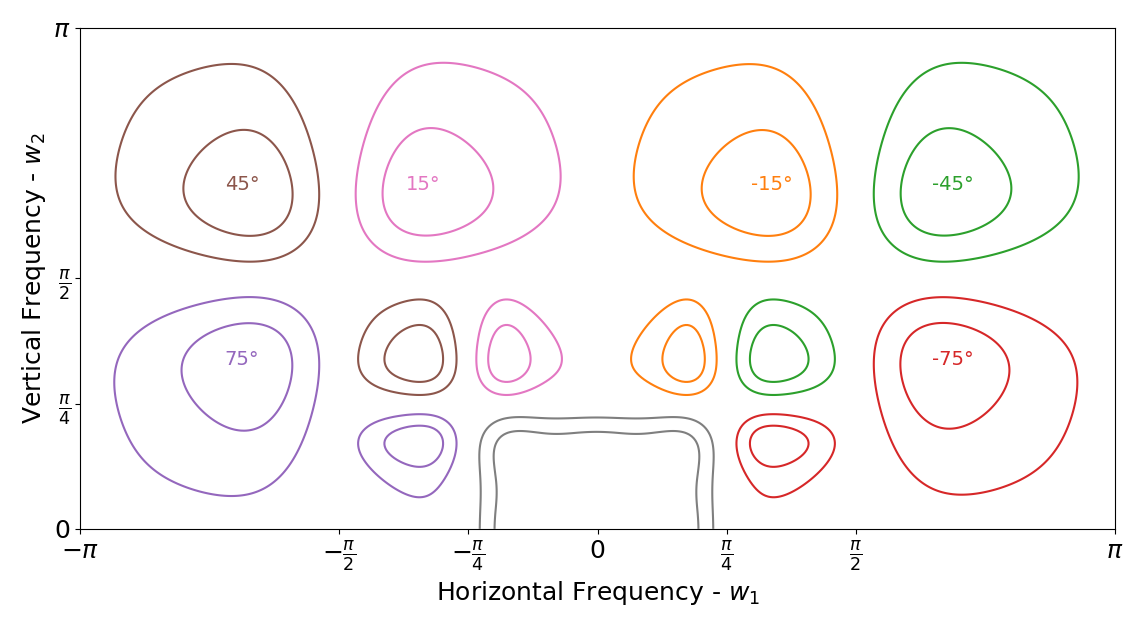
\includegraphics[height=6cm]{\imgpath/subbands.png}
    \label{fig:ch6:dtcwt_bands_freq}
  }
  \hspace{1cm}
%    \newline
  \subfloat[]{%
    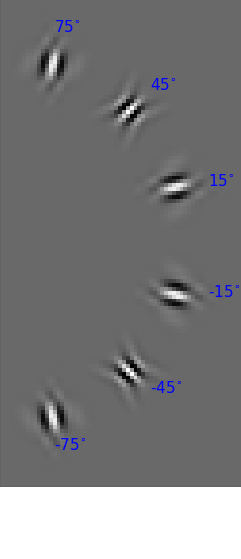
\includegraphics[height=5.7cm]{\imgpath/impulses.png}
    \label{fig:ch6:dtcwt_bands_impulse}
  }
  \mycaption{$\DTCWT$ subbands}{\subref{fig:ch6:dtcwt_bands_freq} -1dB and -3dB contour 
  plots showing the support in the Fourier domain of the 6 subbands of the $\DTCWT$ at scales
  1 and 2, and the scale 2 lowpass. These are the product of the single side-band 
  filters $P(\zz)$ and $Q(\zz)$ from \autoref{thm:ch6:shiftinv}, or half of the
  support of the double side-band filters $A_rS_r + A_iS_i$ and $A_rS_i -
  A_iS_r$ from \eqref{eq:ch6:dtcwt_fwd}.
  \subref{fig:ch6:dtcwt_bands_impulse} The pixel domain impulse responses for
  the second scale wavelets. The Hilbert pair for each wavelet is the underlying
  sinusoid phase shifted by 90 degrees.}
  \label{fig:ch6:dtcwt_bands}
\end{figure}

\subsection{Backpropagation}\label{sec:ch6:dtcwt_update}
Assume we already have access to the quantity $\Delta Y(z)$ (this is the input
to the backwards pass). \autoref{fig:ch6:bwd_pass} illustrates the
backpropagation procedure.

We recall the passthrough and update equations for a convolutional block from
\eqref{eq:ch2:cnn_passthrough} and \eqref{eq:ch2:cnn_weight_update}:
\begin{align}
  \dydx{L}{x_{c,k_1,k_2}} &= \sum_f \Delta y[f, \nn] \star h_c[f, \nn] \\
  \dydx{L}{h_{f,c,k_1,k_2}} &= \Delta y[f, \nn] \star x[c, \nn]
\end{align}
In terms of modified $Z$-transforms, this becomes:
\begin{align}
  \Delta X(c, \zz) &= \sum_f \Delta Y(f, \zz) H'[c, f, \zz^{-1}] \\
  \Delta H(f, c, \zz) &= \sum_f \Delta Y(f, \zz) X[c, \zz^{-1}] 
\end{align}
where $H'$ is
$H$ transposed in the filter and channel dimensions, and $\zz^{-1}$ indicates
the filter was mirror-imaged in the spatial dimension.  %
The simplified, single-channel, single filter, 1-D version of this is:
\begin{align}\label{eq:ch6:backprop}
  \Delta X(z) &=  \Delta Y(z)H(z^{-1}) \\
  \Delta H(z) &=  \Delta Y(z)X(z^{-1})
\end{align}

If H were complex, the first term in \autoref{eq:ch6:backprop} would be
$\bar{H}(1/\bar{z})$, but as each individual block in the $\DTCWT$ of
\autoref{fig:ch6:fwd_bwd} is purely real, we can use the simpler form $H(z^{-1})$. 

We calculate $\Delta V_r(z)$ and $\Delta V_i(z)$ by backpropagating
$\Delta Y(z)$ through the inverse $\DTCWT$. This is the same as doing the
forward $\DTCWT$ on $\Delta Y(z)$ with the synthesis and analysis filters
swapped and time-reversed. Then the weight update equations are:
\begin{align}
  \Delta G_r(z) &= \Delta V_r(z) U_r(z^{-1}) + \Delta V_i(z) U_i(z^{-1})  \label{eq:ch6:gr_update}\\
  \Delta G_i(z) &=  -\Delta V_r(z) U_i(z^{-1}) + \Delta V_i(z) U_r(z^{-1})  \label{eq:ch6:gi_update} 
\end{align}
%
The passthrough equations have similar form to \eqref{eq:ch6:dtcwt_fwd}:
\begin{equation}\label{eq:ch6:dtcwt_passthrough}
    \Delta X(z) = \frac{2\Delta Y(z)}{M} \left[G_r(z^{-M})\left( A_r(z)S_r(z) + A_i(z)S_i(z) \right) + \\
       G_i(z^{-M}) \left(A_r(z)S_i(z) - A_i(z)S_r(z) \right) \right] 
\end{equation}

\subsection{Examples}
\autoref{fig:ch6:examples} shows example impulse responses of the $\DTCWT$ gain
layer. For comparison, we also show similar `impulse responses' for a gain layer
done in the DWT domain\footnote{Modifying DWT coefficients causes a loss of the
alias cancellation properties so these are not true impulse responses.}. The DWT 
outputs come from three random variables: a $1\x 1$ 
convolutional weight applied to each of the low-high, high-low and high-high
subbands. The $\DTCWT$ outputs come from twelve random variables, again a $1\x
1$ convolutional weight, but now applied to six complex subbands. 

To test the space of generated shapes by a vector gain layer gain $g_1$, we
generate $N$ random vectors of length 12, with each entry taken
from a Gaussian distribution with zero mean and
unit variance. We then generate the equivalent point spread functions from
\eqref{eq:ch6:dtcwt_fwd} for the $N$ different instances and measure their 
normalized cross-correlation. We then sort the values and compare the
distribution to a set of $N$ random vectors with $k$ degrees of freedom. 

Our experiments show that the distribution for the $\DTCWT$ gain layer matches
random vectors with roughly 11.5 degrees of freedom (c.f.\ the 12 variables 
the layer has). 
Similarly for the DWT, the normalized cross-correlation matches the distribution for random vectors
with roughly 2.8 degrees of freedom (c.f. 3 random variables in the layer).
This is particularly reassuring for the $\DTCWT$ as it is showing that there is
still representative power despite the redundancy of the transform.

\begin{figure}
  \centering
  \subfloat[]{%
    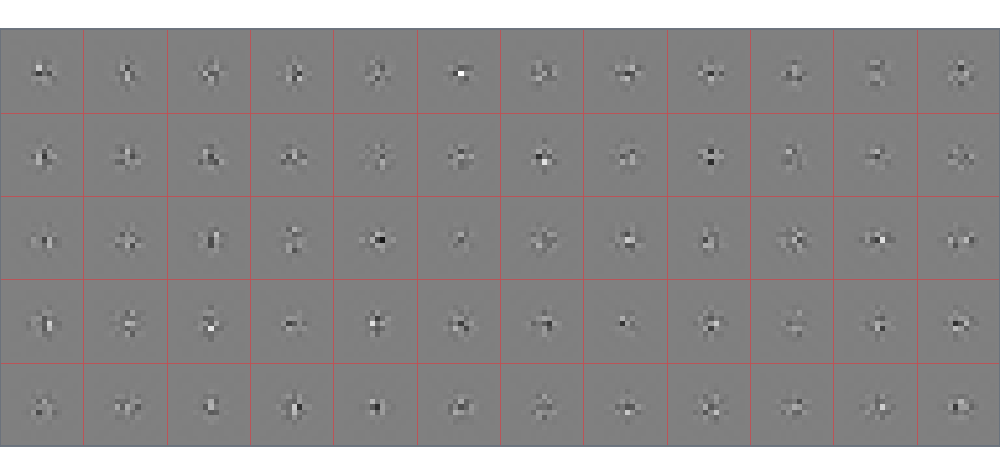
\includegraphics[width=\textwidth]{\imgpath/dtcwt_examples.png}
    \label{fig:ch6:dtcwt_examples}
  }
  \newline
  \subfloat[]{%
  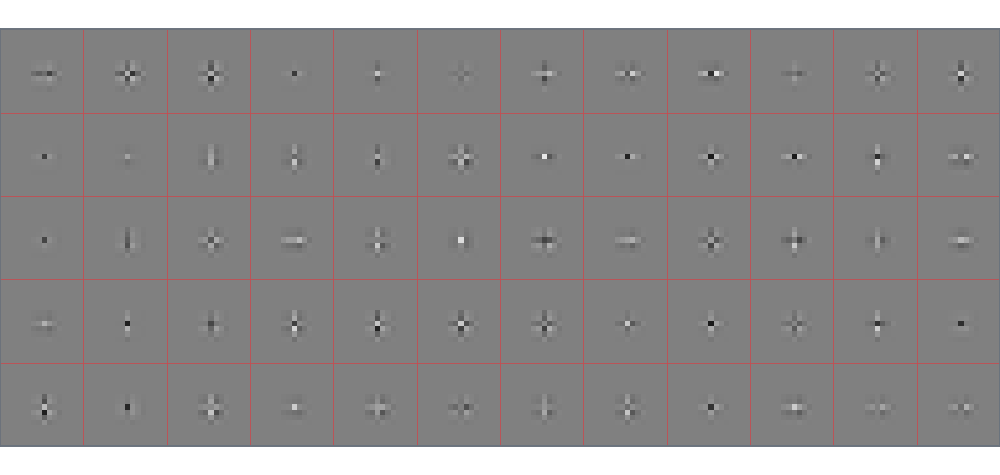
\includegraphics[width=\textwidth]{\imgpath/dwt_examples.png}
    \label{fig:ch6:dwt_examples}
  }
  \mycaption{Example outputs from an impulse input for the proposed gain layers}{
  Example outputs $y = \mathcal{W}^{-1}G\mathcal{W}x$ for an impulse
  $x$ for the $\DTCWT$ gain layer and for a similarly designed DWT gain layer.
  \subref{fig:ch6:dtcwt_examples} shows the output $y$ for a $\DTCWT$ based
  system. $g_{lp} = 0$ and $g_1$ has spatial size $1\x 1$. The 12 values
  in $g_1$ are independently sampled from a random normal of variance 1. 
  The 60 samples come from 60 different random draws of the weights.
  \subref{fig:ch6:dwt_examples}
  shows the outputs $y$ when $x$ is an impulse and $\mathcal{W}$ is the DWT with a
  `db2' wavelet family. Here 3 random numbers are generated for the $g_1$
  coefficients. The strong horizontal and vertical properties of the DWT
  can clearly be seen in comparison to the much freer $\DTCWT$.}
  \label{fig:ch6:examples}
\end{figure}


\subsection{Implementation Details}
Before analyzing its performance, we compare the implementation properties of
our proposed layer to a standard convolutional layer.

\subsubsection{Parameter Memory Cost}\label{sec:ch6:memory}
A standard convolutional layer with $C_l$ input channels, $C_{l+1}$ output channels
and kernel size $k\x k$ has $k^2C_{l}C_{l+1}$ parameters, with $k=3$ or $k=5$
common choices for the spatial size.
\begin{equation}
  \text{\#conv params} = k^2C_lC_{l+1}
\end{equation}

We must choose the spatial sizes of both the lowpass and bandpass
mixing kernels. In our work, we are somewhat limited in how large we would like
to set the bandpass spatial size, as every extra pixel of support requires $2\x
6=12$ extra parameters. For this reason, we almost always set it to have 
support $1\x 1$. The lowpass gains are less costly, and we are free to set them to size
$k_{lp}\x k_{lp}$ (with $k_{lp} = 1,3,5$ in many of our experiments).
%
Further, due to the size of the datasets we test on, we typically limit
ourselves initially to only considering a single scale. If we wish, we can
decompose the input into more scales, resulting in a larger net area of effect.
In particular, it may be useful to do a two-scale transform and discard the
first scale coefficients. This does not increase the number of gains to learn
but changes the position of the bands in the frequency space.

The number of parameters for the gain layer with $k_{lp}=1$ is:
\begin{equation}
  \text{\#params} = (2\x 6 + 1)C_lC_{l+1} = 13C_lC_{l+1} \label{eq:ch6:memcost2}
\end{equation} 
%
This is slightly larger than the $9C_lC_{l+1}$ parameters used in a
standard $3\x 3$ convolution, but as \autoref{fig:ch6:examples} shows, the
spatial support of the full filter is larger than an equivalent one
parameterized in the filter domain. If $k_{lp}=3$ then we would have $21C_l
C_{l+1}$ parameters, slightly fewer than the $25C_l C_{l+1}$ of a $5\x 5$ convolution.

\subsubsection{Activation Memory Cost}\label{sec:ch6:act_memory}
A standard convolutional layer needs to save the activation $x^{(l)}$ to
convolve with the backpropagated gradient $\dydx{L}{y^{(l+1)}}$ on the backwards
pass (to give $\dydx{L}{w^{(l)}}$). For an input with $C_l$ channels of spatial
size $H\x W$, this means
%
\begin{equation}
  \text{\#conv floats} = HWC_l 
\end{equation}

Our layer requires us to save the wavelet coefficients $u_{lp}$ and $u_{j,k}$
for updating the $g$ terms as in \eqref{eq:ch6:gr_update} and \eqref{eq:ch6:gi_update}.  
For the $4:1$ redundant $\DTCWT$, this requires:
%
\begin{equation}
  \text{\#$\DTCWT$ floats} = 4HWC_l 
\end{equation}
%
to be saved for the backwards pass.  You can see this difference from the
difference in the block diagrams in \autoref{fig:ch6:block_diagrams}.

Note that a single scale $\DTCWT$ gain layer requires $16/7$ times as many
floats to be saved as compared to the invariant layer of the previous chapter.
The extra cost of this comes from two things. Firstly, we keep the real and
imaginary components for the bandpass (as opposed to only the magnitude),
meaning we need $3HWC_l$ floats, rather than $\frac{3}{2}HWC_l$. Additionally,
the lowpass was downsampled in the previous chapter, requiring only
$\frac{1}{4}HWC_l$, whereas we keep the full sample rate, costing $HWC_l$.

If memory is an issue and the computation of the $\DTCWT$ is very fast, then we
only need to save the $x^{(l)}$ coefficients and can calculate the $u$'s on the
fly during the backwards pass. Note that a two-scale $\DTCWT$ gain layer would
still only require $4HWC_l$ floats.

\subsubsection{Computational Cost}\label{sec:ch6:computation}
A standard convolutional layer with kernel size $k\x k$ needs $k^2C_{l+1}$
multiplies per input pixel (of which there are $C_{l}\x H\x W$).

For the $\DTCWT$, the overhead calculations are the same as in
\autoref{sec:ch5:computation}, so we will omit their derivation here. The mixing
is however different, requiring complex convolution for the bandpass
coefficients, and convolution over a higher resolution lowpass. The bandpass has
one quarter spatial resolution at the first scale, but this is offset by the
$4:1$ cost of complex multiplies compared to real multiplies. Again assuming we
have set $J=1$ and $k_{lp} = 1$ then the total cost for the gain layer is:
%
\begin{equation}
  % \frac{7}{4}C_{l+1} + 48 \label{eq:comp}
  \text{\#mults/pixel} = \underbrace{\hphantom{1} \frac{6\x 4}{4}C_{l+1} \hphantom{1}}_{\textrm{bandpass}} +
  \underbrace{\hphantom{1}\vphantom{\frac{6}{4}} C_{l+1} \hphantom{1}}_{\textrm{lowpass}} + 
  \underbrace{\vphantom{\frac{6}{4}} 36}_{\DTCWT} + 
  \underbrace{\vphantom{\frac{6}{4}} 36}_{\DTCWT^{-1}} = \quad 7C_{l+1} + 72 \quad
  \label{eq:ch6:comp_dtcwt}
\end{equation}
which is marginally smaller than the $9C_{l+1}$ of a $3\x 3$ convolutional layer (if $C_{l+1}$ > 36).

\subsubsection{Parameter Initialization}
For both layer types we use the Glorot Initialization scheme \cite{glorot_understanding_2010}
with $a=1$: 
%
\begin{equation}
  g_{ij} \drawnfrom U\left[ -\sqrt{\frac{6}{(C_l + C_{l+1})k^2}},\ \sqrt{\frac{6}{(C_l + C_{l+1})k^2}}\
  \right] \label{eq:ch6:glorot}
\end{equation}
where $k$ is the kernel size.
